\documentclass{beamer}
\usepackage{../../shared/styles/custom}
\usepackage{../../shared/styles/conventions}

% Add slide numbers with total
\setbeamertemplate{footline}{
  \hfill%
  \usebeamercolor[fg]{page number in head/foot}%
  \usebeamerfont{page number in head/foot}%
  \insertframenumber\,/\,\inserttotalframenumber\kern1em\vskip2pt%
}

\title{Precision-Recall Curves and Evaluation Metrics}
\date{\today}
\author{Nipun Batra}
\institute{IIT Gandhinagar}

\begin{document}
\maketitle

\begin{frame}{Table of Contents}
\tableofcontents
\end{frame}

\section{Motivation: Real-World Application}

\begin{frame}{Brick Kiln Detection from Satellite Imagery}
\begin{center}
\textbf{Problem:} Identify illegal brick kilns using satellite imagery
\end{center}

\vspace{0.15cm}

\begin{keypointsbox}{Why This Matters}
\small
\begin{itemize}
    \item Environmental monitoring and air quality
    \item Thousands of square kilometers to survey
    \item Manual inspection is infeasible
\end{itemize}
\end{keypointsbox}
\end{frame}

\begin{frame}{The Challenge: Scale of the Problem}
\begin{block}{Dataset Scale}
\begin{itemize}
    \item \textbf{Images to scan:} 10,000 satellite images
    \item \textbf{Manual inspection time:} 30 seconds per image
    \item \textbf{Total manual effort:} $10{,}000 \times 30s$
    \item \textbf{That's 83 hours of continuous work!}
\end{itemize}
\end{block}

\vspace{0.2cm}

\begin{center}
\Large
Can we automate this with machine learning?
\end{center}
\end{frame}

\begin{frame}{Why Not Just Use Accuracy?}
\begin{alertblock}{Three Models to Choose From}
\small
\begin{itemize}
    \item Model A: 95\% accuracy
    \item Model B: 92\% accuracy
    \item Model C: 89\% accuracy
\end{itemize}
\end{alertblock}

\vspace{0.2cm}
\pause

\begin{keypointsbox}{The Problem}
\small
Accuracy doesn't tell us about the \textbf{types of errors}!
\end{keypointsbox}
\end{frame}

\begin{frame}{Types of Errors Matter}
\begin{examplebox}{False Positive (Type I Error)}
\small
Model says ``brick kiln detected'' but there isn't one
\begin{itemize}
    \item Wastes inspector's time
    \item Reduces trust in the system
\end{itemize}
\end{examplebox}

\vspace{0.15cm}

\begin{examplebox}{False Negative (Type II Error)}
\small
Model misses an actual brick kiln
\begin{itemize}
    \item Environmental violation goes undetected
    \item Defeats the purpose of monitoring
\end{itemize}
\end{examplebox}
\end{frame}

\begin{frame}{Scenario 1: High Precision Model}
\footnotesize
\begin{examplebox}{Conservative Classifier}
\small
\textbf{Model behavior:} Only flags when very confident
\end{examplebox}

\begin{block}{Results}
\begin{itemize}
    \item Flags 100 images as ``has brick kiln''
    \item Inspector time: $100 \times 30s = 50$ minutes
\end{itemize}
\end{block}

\begin{keypointsbox}{Trade-offs}
\small
\begin{itemize}
    \item[\textcolor{green}{\checkmark}] Few false alarms
    \item[\textcolor{green}{\checkmark}] Inspector time well-spent
    \item[\textcolor{red}{$\times$}] Might miss many kilns
\end{itemize}
\end{keypointsbox}
\end{frame}

\begin{frame}{Scenario 2: High Recall Model}
\footnotesize
\begin{examplebox}{Aggressive Classifier}
\small
\textbf{Model behavior:} Flags anything suspicious
\end{examplebox}

\begin{block}{Results}
\begin{itemize}
    \item Flags 2,000 images as ``has brick kiln''
    \item Inspector time: $2{,}000 \times 30s = 16.7$ hours
\end{itemize}
\end{block}

\begin{keypointsbox}{Trade-offs}
\small
\begin{itemize}
    \item[\textcolor{green}{\checkmark}] Catches almost all kilns
    \item[\textcolor{red}{$\times$}] Many false alarms
    \item[\textcolor{red}{$\times$}] Wastes inspector time
\end{itemize}
\end{keypointsbox}
\end{frame}

\section{Classification Metrics Fundamentals}

\begin{frame}{The Confusion Matrix}
\begin{columns}
\begin{column}{0.48\textwidth}
\begin{definitionbox}{Confusion Matrix}
\small
\begin{center}
\begin{tabular}{cc|c|c|}
& \multicolumn{1}{c}{} & \multicolumn{2}{c}{Predicted} \\
& \multicolumn{1}{c}{} & \multicolumn{1}{c}{Pos} & \multicolumn{1}{c}{Neg} \\
\cline{3-4}
\multirow{2}{*}{\rotatebox{90}{Actual}} & Pos & TP & FN \\
\cline{3-4}
& Neg & FP & TN \\
\cline{3-4}
\end{tabular}
\end{center}
\end{definitionbox}

\vspace{0.2cm}

\small
\begin{itemize}
    \item \textbf{TP}: Correct positive
    \item \textbf{FP}: Type I error
    \item \textbf{TN}: Correct negative
    \item \textbf{FN}: Type II error
\end{itemize}
\end{column}
\begin{column}{0.48\textwidth}
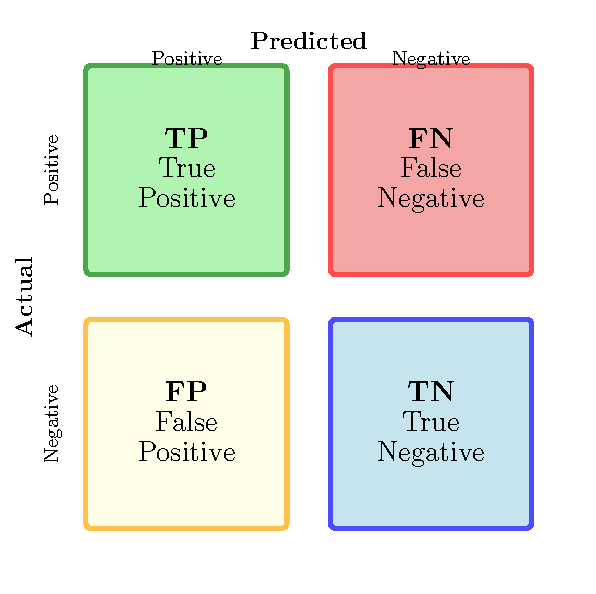
\includegraphics[width=\textwidth]{confusion-matrix-diagram.pdf}
\end{column}
\end{columns}
\end{frame}

\begin{frame}{Precision: Reliability of Positive Predictions}
\begin{definitionbox}{Precision}
\small
$$\text{Precision} = \frac{\text{TP}}{\text{TP} + \text{FP}}$$

\vspace{0.2cm}

\textbf{Question it answers:} \\
Of all instances we predicted as positive, \\
what fraction was actually positive?
\end{definitionbox}
\end{frame}

\begin{frame}{Precision: Example}
\begin{examplebox}{Brick Kiln Detection}
\small
\begin{itemize}
    \item Model flags 100 images as having brick kilns
    \item 80 actually have brick kilns (TP)
    \item 20 are false alarms (FP)
\end{itemize}

\vspace{0.2cm}

$$\text{Precision} = \frac{80}{100} = 0.80 \text{ or } 80\%$$
\end{examplebox}

\vspace{0.2cm}

\begin{keypointsbox}{Interpretation}
\small
When the model says ``brick kiln detected,'' it's correct 80\% of the time
\end{keypointsbox}
\end{frame}

\begin{frame}{Recall: Completeness of Detection}
\begin{definitionbox}{Recall (Sensitivity, TPR)}
\small
$$\text{Recall} = \frac{\text{TP}}{\text{TP} + \text{FN}}$$

\vspace{0.2cm}

\textbf{Question it answers:} \\
Of all actual positive instances, \\
what fraction did we correctly identify?
\end{definitionbox}
\end{frame}

\begin{frame}{Recall: Example}
\begin{examplebox}{Brick Kiln Detection}
\small
\begin{itemize}
    \item 150 images actually contain brick kilns
    \item Model correctly identifies 80 (TP)
    \item Model misses 70 of them (FN)
\end{itemize}

\vspace{0.2cm}

$$\text{Recall} = \frac{80}{150} = 0.533 \text{ or } 53.3\%$$
\end{examplebox}

\vspace{0.2cm}

\begin{keypointsbox}{Interpretation}
\small
The model finds only about half of all brick kilns
\end{keypointsbox}
\end{frame}

\begin{frame}{The Precision-Recall Trade-off}
\begin{keypointsbox}{Fundamental Tension}
\small
Improving one metric often hurts the other!
\end{keypointsbox}

\vspace{0.2cm}

\begin{center}
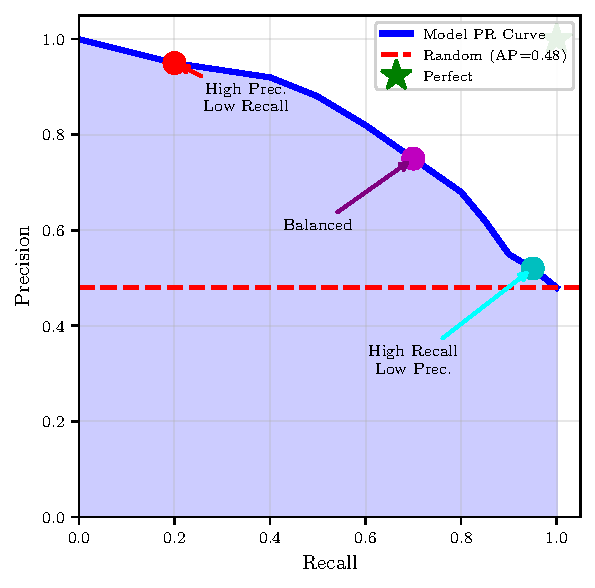
\includegraphics[width=0.55\textwidth]{pr-curve-diagram.pdf}
\end{center}
\end{frame}

\begin{frame}{Trade-off: Model Behavior}
\begin{columns}
\begin{column}{0.48\textwidth}
\begin{block}{Conservative Model}
\begin{itemize}
    \item High threshold
    \item Few predictions
    \item High precision
    \item Low recall
\end{itemize}
\end{block}
\end{column}

\begin{column}{0.48\textwidth}
\begin{block}{Aggressive Model}
\begin{itemize}
    \item Low threshold
    \item Many predictions
    \item Low precision
    \item High recall
\end{itemize}
\end{block}
\end{column}
\end{columns}
\end{frame}

\section{Classification Thresholds}

\begin{frame}{From Probabilities to Predictions}
\begin{columns}
\begin{column}{0.48\textwidth}
\begin{definitionbox}{How Classifiers Work}
\small
Most classifiers output \textbf{probabilities}, not direct predictions

\vspace{0.15cm}

Classification threshold $\tau$ converts probabilities to classes:
$$\hat{y} = \begin{cases}
1 & \text{if } P(y=1|x) \geq \tau \\
0 & \text{if } P(y=1|x) < \tau
\end{cases}$$

Default: $\tau = 0.5$
\end{definitionbox}
\end{column}
\begin{column}{0.52\textwidth}
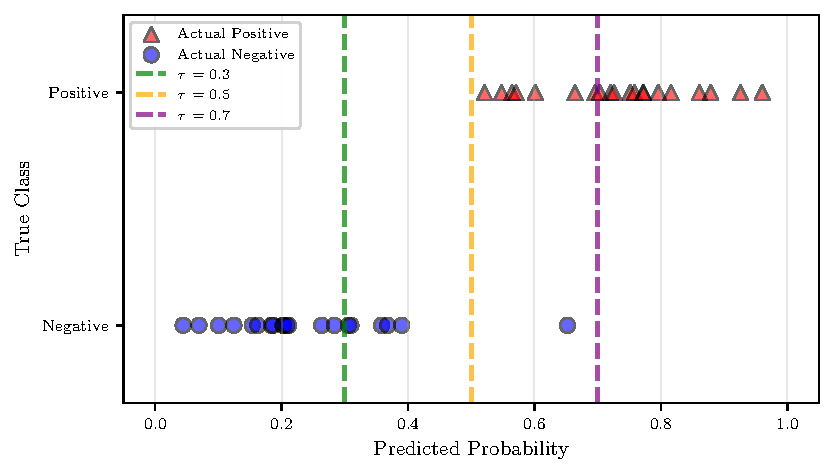
\includegraphics[width=\textwidth]{threshold-effect-diagram.pdf}
\end{column}
\end{columns}
\end{frame}

\begin{frame}{Threshold Example}
\begin{examplebox}{Three Images, Different Thresholds}
\small
\begin{center}
\begin{tabular}{|c|c|c|c|}
\hline
Image & $P(\text{kiln})$ & $\tau=0.5$ & $\tau=0.7$ \\
\hline
A & 0.85 & Positive & Positive \\
B & 0.62 & Positive & \textcolor{red}{Negative} \\
C & 0.38 & Negative & Negative \\
\hline
\end{tabular}
\end{center}
\end{examplebox}

\vspace{0.15cm}

\begin{keypointsbox}{Key Insight}
\small
Same model, different thresholds = different predictions!
\end{keypointsbox}
\end{frame}

\begin{frame}{Low Threshold Effects}
\begin{block}{Threshold $\tau = 0.3$}
Classify as positive if $P(y=1|x) \geq 0.3$
\end{block}

\vspace{0.15cm}

\begin{itemize}
    \item More instances classified as positive
    \item \textcolor{green}{Higher recall} (catch more positives)
    \item \textcolor{red}{Lower precision} (more false positives)
    \item More false alarms
\end{itemize}

\vspace{0.15cm}

\begin{center}
\textbf{Use when:} Missing positives is costly
\end{center}
\end{frame}

\begin{frame}{High Threshold Effects}
\begin{block}{Threshold $\tau = 0.7$}
Classify as positive if $P(y=1|x) \geq 0.7$
\end{block}

\vspace{0.15cm}

\begin{itemize}
    \item Fewer instances classified as positive
    \item \textcolor{red}{Lower recall} (miss more positives)
    \item \textcolor{green}{Higher precision} (fewer false positives)
    \item Fewer false alarms
\end{itemize}

\vspace{0.15cm}

\begin{center}
\textbf{Use when:} False alarms are costly
\end{center}
\end{frame}

\section{Precision-Recall Curves}

\begin{frame}{What is a PR Curve?}
\footnotesize
\begin{columns}
\begin{column}{0.48\textwidth}
\begin{definitionbox}{Precision-Recall Curve}
\small
A plot showing precision vs. recall for all possible threshold values

\vspace{0.15cm}

\begin{itemize}
    \item \textbf{X-axis:} Recall
    \item \textbf{Y-axis:} Precision
    \item Each point = one threshold value
\end{itemize}
\end{definitionbox}
\begin{keypointsbox}{What It Shows}
The complete trade-off space between precision and recall
\end{keypointsbox}
\end{column}
\begin{column}{0.48\textwidth}
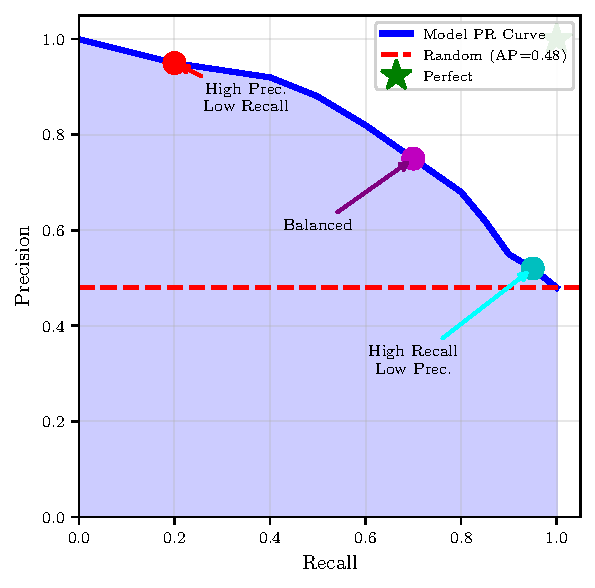
\includegraphics[width=\textwidth]{pr-curve-diagram.pdf}
\end{column}
\end{columns}
\end{frame}

\begin{frame}{Building a PR Curve: Steps}
\begin{enumerate}
    \item Train classifier (e.g., Logistic Regression)

    \vspace{0.15cm}

    \item Get predicted probabilities for test set

    \vspace{0.15cm}

    \item For each threshold $\tau \in [0, 1]$:
    \begin{itemize}
        \item Apply threshold to get predictions
        \item Compute confusion matrix
        \item Calculate precision and recall
        \item Plot (recall, precision) point
    \end{itemize}
\end{enumerate}
\end{frame}

\begin{frame}{Building a PR Curve: Visualization}
\begin{center}
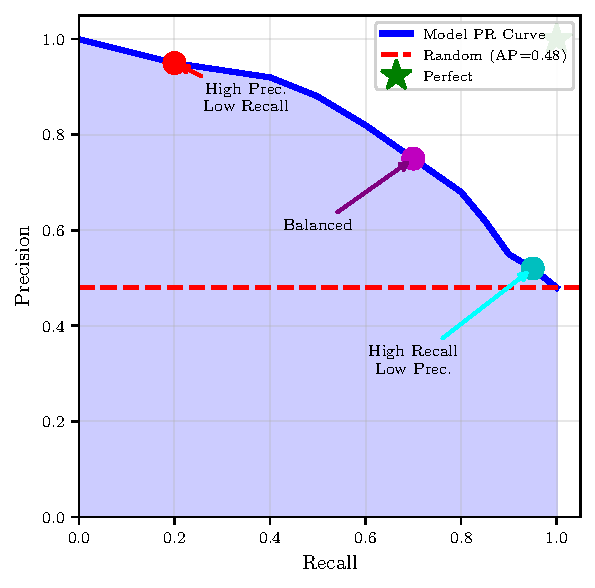
\includegraphics[width=0.8\textwidth]{pr-curve-diagram.pdf}
\end{center}

\vspace{0.15cm}

\begin{keypointsbox}{Result}
\small
Connect all threshold points to form the complete PR curve
\end{keypointsbox}
\end{frame}

\begin{frame}[fragile]{Implementation in Scikit-learn}
\begin{block}{Python Code}
\begin{verbatim}
from sklearn.metrics import precision_recall_curve

# Get predicted probabilities
y_scores = model.predict_proba(X_test)[:, 1]

# Compute PR curve
precision, recall, thresholds = \
    precision_recall_curve(y_test, y_scores)
\end{verbatim}
\end{block}
\end{frame}

\begin{frame}{Example: Synthetic Dataset}
\begin{examplebox}{Dataset from Notebook}
\small
\begin{itemize}
    \item Created using \texttt{make\_blobs()}
    \item 100 samples, 2 features, 2 classes
    \item Training: 40 samples
    \item Test: 60 samples
    \item Cluster standard deviation: 8.0
    \item Classifier: Logistic Regression
\end{itemize}
\end{examplebox}
\end{frame}

\begin{frame}{Threshold Analysis: Low Values}
\begin{examplebox}{From Notebook: Threshold = 0.00}
\small
\begin{itemize}
    \item \textbf{Precision:} 0.48
    \item \textbf{Recall:} 1.00
\end{itemize}

\vspace{0.2cm}

\textbf{Interpretation:}
\begin{itemize}
    \item Classifies almost everything as positive
    \item Catches all positive cases (perfect recall)
    \item But only 48\% are actually positive
\end{itemize}
\end{examplebox}
\end{frame}

\begin{frame}{Threshold Analysis: Medium Values}
\begin{examplebox}{From Notebook: Threshold = 0.50}
\small
\begin{itemize}
    \item \textbf{Precision:} 0.74
    \item \textbf{Recall:} 0.69
\end{itemize}

\vspace{0.2cm}

\textbf{Interpretation:}
\begin{itemize}
    \item Balanced operating point
    \item Good precision: 74\% of predictions correct
    \item Good recall: finds 69\% of positives
    \item This is the default threshold
\end{itemize}
\end{examplebox}
\end{frame}

\begin{frame}{Threshold Analysis: High Values}
\begin{examplebox}{From Notebook: Threshold = 0.90}
\small
\begin{itemize}
    \item \textbf{Precision:} 1.00
    \item \textbf{Recall:} 0.24
\end{itemize}

\vspace{0.2cm}

\textbf{Interpretation:}
\begin{itemize}
    \item Very conservative classification
    \item Perfect precision: all predictions correct!
    \item But misses 76\% of positive cases
    \item Only confident predictions are made
\end{itemize}
\end{examplebox}
\end{frame}

\begin{frame}{Complete Threshold Table}
\begin{columns}
\begin{column}{0.48\textwidth}
\begin{center}
\small
\begin{tabular}{|c|c|c|}
\hline
\textbf{Threshold} & \textbf{Precision} & \textbf{Recall} \\
\hline
0.00 & 0.48 & 1.00 \\
\hline
0.10 & 0.55 & 0.98 \\
\hline
0.30 & 0.65 & 0.85 \\
\hline
0.50 & 0.74 & 0.69 \\
\hline
0.70 & 0.85 & 0.45 \\
\hline
0.90 & 1.00 & 0.24 \\
\hline
\end{tabular}
\end{center}
\end{column}
\begin{column}{0.48\textwidth}
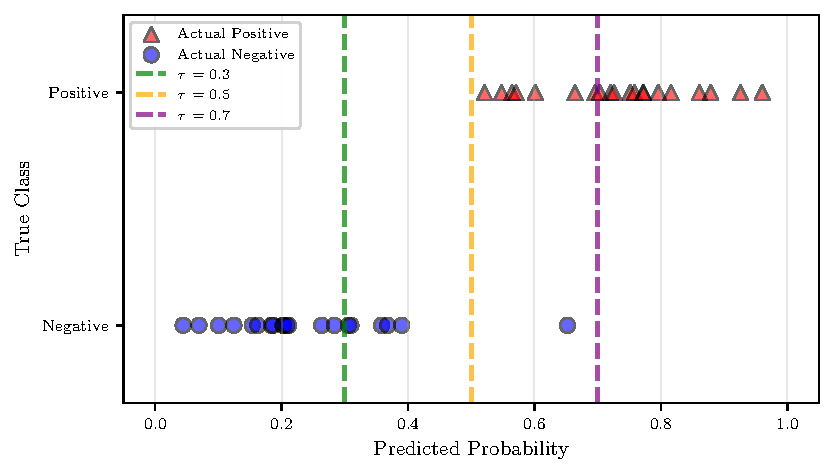
\includegraphics[width=\textwidth]{threshold-effect-diagram.pdf}
\end{column}
\end{columns}

\vspace{0.2cm}

\begin{keypointsbox}{Observation}
\small
As threshold increases: Precision $\uparrow$, Recall $\downarrow$
\end{keypointsbox}
\end{frame}

\begin{frame}{Interpreting PR Curves}
\begin{center}
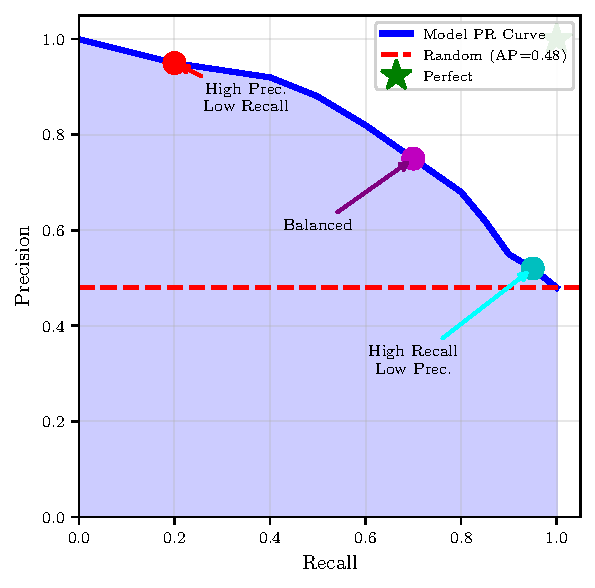
\includegraphics[width=0.8\textwidth]{pr-curve-diagram.pdf}
\end{center}

\end{frame}

\begin{frame}{Interpreting PR Curves}
\begin{keypointsbox}{What Makes a Good Curve?}
\begin{itemize}
    \item Curve closer to top-right is better
    \item Top-right = high precision AND high recall
    \item Perfect classifier: stays at $(1, 1)$
\end{itemize}
\end{keypointsbox}
\end{frame}

\begin{frame}{Interpreting PR Curves: Baseline}
\begin{block}{Baseline: Random Classifier}
Horizontal line at $y = \frac{\text{\# positives}}{\text{total}}$

\vspace{0.15cm}

For balanced classes: $y = 0.5$
\end{block}

\vspace{0.2cm}

\begin{examplebox}{Example}
\small
If 48\% of data is positive class: \\
Random classifier has precision $\approx 0.48$ at all recall levels
\end{examplebox}
\end{frame}

\begin{frame}{Comparing Models with PR Curves}
\begin{alertblock}{Model Comparison Rules}
\small
\begin{enumerate}
    \item If one curve dominates (always above), \\
          that model is better

    \vspace{0.15cm}

    \item If curves cross, choice depends on your needs:
    \begin{itemize}
        \item Need high precision? Use left side of curve
        \item Need high recall? Use right side of curve
    \end{itemize}
\end{enumerate}
\end{alertblock}

\vspace{0.15cm}

\begin{center}
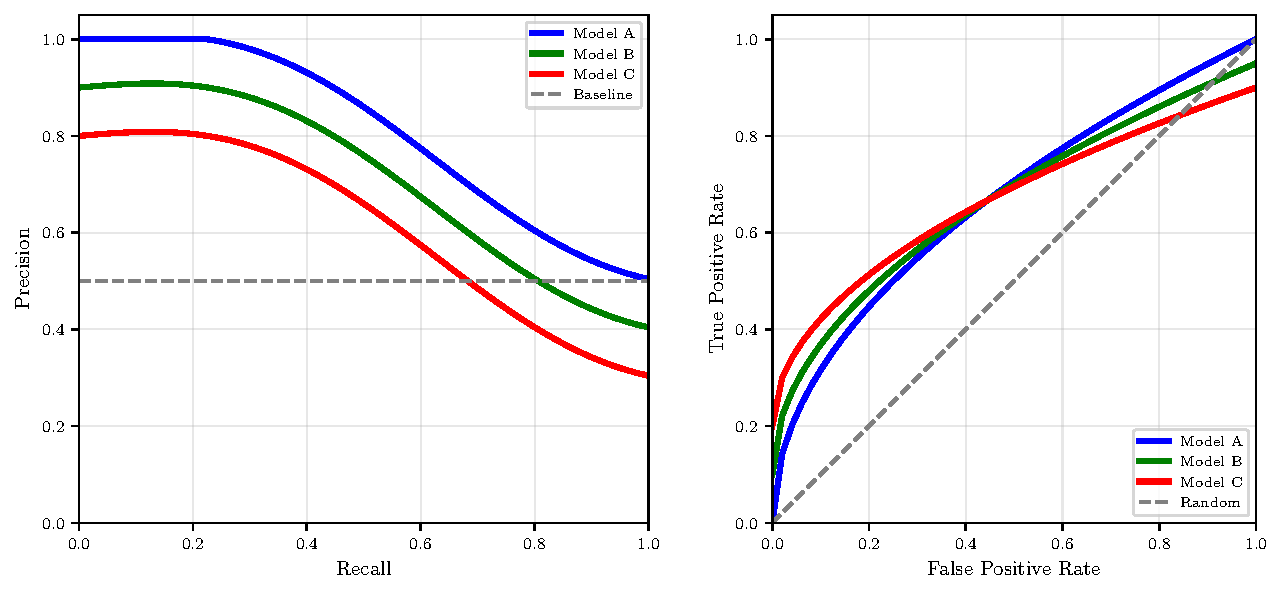
\includegraphics[width=0.6\textwidth]{model-comparison-diagram.pdf}
\end{center}
\end{frame}

\section{Application-Specific Decisions}

\begin{frame}{When to Prioritize Precision}
\begin{examplebox}{High Precision Scenarios}
\small
False positives are costly:
\end{examplebox}

\vspace{0.15cm}

\begin{itemize}
    \item \textbf{Spam detection} \\
          Don't want legitimate emails in spam folder

    \item \textbf{Medical diagnosis} \\
          Before expensive/risky treatment

    \item \textbf{Fraud detection} \\
          Don't block legitimate transactions
\end{itemize}

\vspace{0.15cm}

\begin{center}
\textbf{Strategy:} Choose high threshold
\end{center}
\end{frame}

\begin{frame}{When to Prioritize Recall}
\begin{examplebox}{High Recall Scenarios}
\small
False negatives are costly:
\end{examplebox}

\vspace{0.15cm}

\begin{itemize}
    \item \textbf{Cancer screening} \\
          Can't afford to miss cases

    \item \textbf{Security threats} \\
          Missing a threat is catastrophic

    \item \textbf{Environmental compliance} \\
          Must catch all violations
\end{itemize}

\vspace{0.15cm}

\begin{center}
\textbf{Strategy:} Choose low threshold
\end{center}
\end{frame}

\begin{frame}{Decision Analysis: Option A}
\begin{block}{High Precision Choice: $\tau = 0.7$}
\textbf{Metrics:}
\begin{itemize}
    \item Precision: 0.85
    \item Recall: 0.55
\end{itemize}
\end{block}

\vspace{0.15cm}

\begin{examplebox}{Implications}
\small
\begin{itemize}
    \item Flags 200 images
    \item 170 true positives, 30 false positives
    \item Inspection time: 1.7 hours
    \item \textcolor{red}{Misses 45\% of kilns}
\end{itemize}
\end{examplebox}
\end{frame}

\begin{frame}{Decision Analysis: Option B}
\begin{block}{High Recall Choice: $\tau = 0.4$}
\textbf{Metrics:}
\begin{itemize}
    \item Precision: 0.65
    \item Recall: 0.85
\end{itemize}
\end{block}

\vspace{0.15cm}

\begin{examplebox}{Implications}
\small
\begin{itemize}
    \item Flags 500 images
    \item 325 true positives, 175 false positives
    \item Inspection time: 4.2 hours
    \item \textcolor{green}{Only misses 15\% of kilns}
\end{itemize}
\end{examplebox}
\end{frame}

\begin{frame}{Which Option to Choose?}
\begin{alertblock}{Decision Factors}
\small
\begin{itemize}
    \item \textbf{Budget:} How much inspector time available?
    \item \textbf{Legal:} Required detection rate?
    \item \textbf{Environmental urgency:} Cost of missed kilns?
\end{itemize}
\end{alertblock}

\vspace{0.15cm}

\begin{keypointsbox}{Typical Choice}
\small
For environmental compliance: \\
Option B (high recall) is usually preferred

\vspace{0.2cm}

Missing violations is worse than \\
spending extra inspection time
\end{keypointsbox}
\end{frame}

\section{Related Metrics}

\begin{frame}{F1 Score: Balancing Both Metrics}
\begin{definitionbox}{F1 Score}
\small
Harmonic mean of precision and recall:

$$F_1 = 2 \cdot \frac{\text{Precision} \cdot \text{Recall}}{\text{Precision} + \text{Recall}}$$

\vspace{0.2cm}

Alternative form:
$$F_1 = \frac{2 \cdot \text{TP}}{2 \cdot \text{TP} + \text{FP} + \text{FN}}$$
\end{definitionbox}
\end{frame}

\begin{frame}{Why Harmonic Mean?}
\begin{keypointsbox}{Properties of F1}
\small
\begin{itemize}
    \item Range: $[0, 1]$, higher is better
    \item Heavily penalizes imbalanced metrics
    \item Both precision and recall must be good
\end{itemize}
\end{keypointsbox}

\vspace{0.15cm}

\begin{examplebox}{Example Comparison}
\small
\begin{itemize}
    \item $P=0.80, R=0.60 \Rightarrow F_1 = 0.686$
    \item $P=0.70, R=0.70 \Rightarrow F_1 = 0.700$
\end{itemize}

Balanced metrics give better F1!
\end{examplebox}
\end{frame}

\begin{frame}{$F_\beta$ Score: Weighted Version}
\begin{definitionbox}{$F_\beta$ Score}
\small
$$F_\beta = (1 + \beta^2) \cdot \frac{\text{Precision} \cdot \text{Recall}}{\beta^2 \cdot \text{Precision} + \text{Recall}}$$

\vspace{0.2cm}

\textbf{Parameter $\beta$:}
\begin{itemize}
    \item $\beta = 1$: Equal weight ($F_1$ score)
    \item $\beta < 1$: Favor precision (e.g., $F_{0.5}$)
    \item $\beta > 1$: Favor recall (e.g., $F_2$)
\end{itemize}
\end{definitionbox}
\end{frame}

\begin{frame}{$F_\beta$ Applications: High Recall}
\begin{examplebox}{$F_2$ Score}
\small
\textbf{Use when:} Recall is 2× more important than precision

\vspace{0.15cm}

\textbf{Applications:}
\begin{itemize}
    \item \textbf{Cancer screening} \\
          Missing a cancer case is catastrophic

    \vspace{0.2cm}

    \item \textbf{Security threat detection} \\
          Can't afford to miss threats

    \vspace{0.2cm}

    \item \textbf{Environmental compliance} \\
          Our brick kiln detection example
\end{itemize}
\end{examplebox}

\vspace{0.15cm}

\begin{center}
Higher $\beta$ = More weight on recall
\end{center}
\end{frame}

\begin{frame}{$F_\beta$ Applications: High Precision}
\begin{examplebox}{$F_{0.5}$ Score}
\textbf{Use when:} Precision is 2× more important than recall

\vspace{0.15cm}

\textbf{Applications:}
\begin{itemize}
    \item \textbf{Search engines} \\
          Show most relevant results first

    \vspace{0.2cm}

    \item \textbf{Spam detection} \\
          Avoid false positives (legitimate emails in spam)

    \vspace{0.2cm}

    \item \textbf{Medical diagnoses} \\
          Before expensive/invasive treatments
\end{itemize}
\end{examplebox}

\vspace{0.15cm}

\begin{center}
Lower $\beta$ = More weight on precision
\end{center}
\end{frame}

\begin{frame}{Average Precision (AP)}
\begin{definitionbox}{Average Precision}
\small
Area under the precision-recall curve:

$$\text{AP} = \sum_{n=1}^{N} (R_n - R_{n-1}) \cdot P_n$$

where $P_n$ and $R_n$ are precision and recall \\
at the $n$-th threshold
\end{definitionbox}

\vspace{0.15cm}

\begin{center}
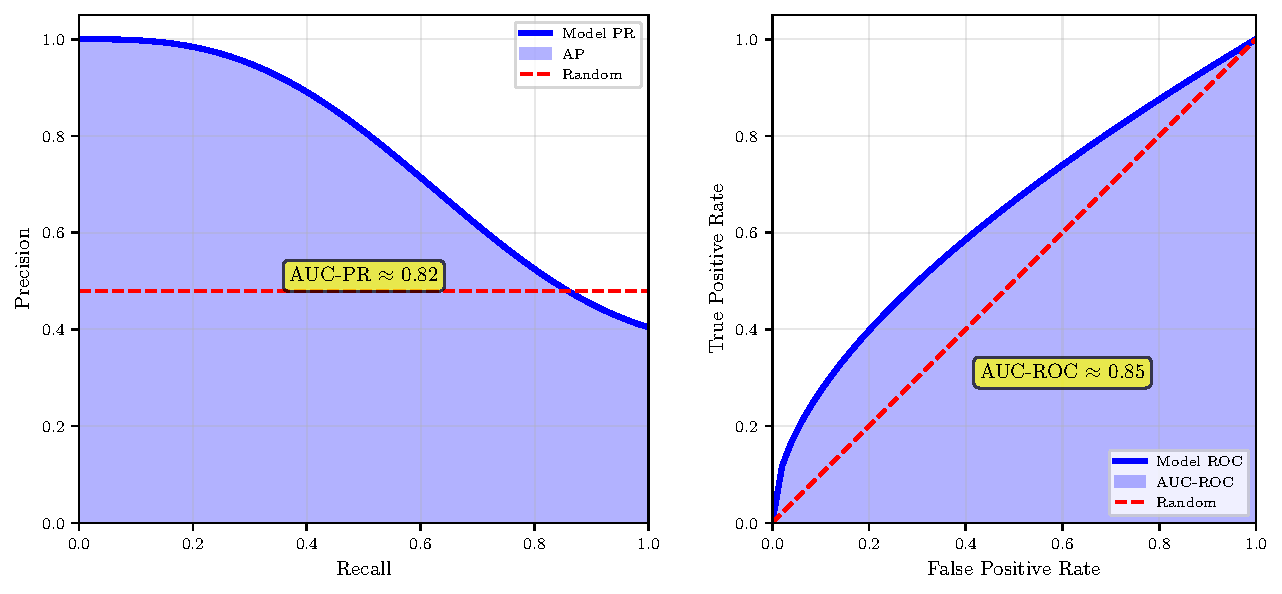
\includegraphics[width=0.6\textwidth]{auc-diagram.pdf}
\end{center}
\end{frame}

\begin{frame}{Average Precision: Properties}
\begin{keypointsbox}{Key Properties}
\small
\begin{itemize}
    \item Range: $[0, 1]$, higher is better
    \item Single number summarizing entire curve
    \item Perfect classifier: $\text{AP} = 1.0$
    \item Weighted by recall changes
\end{itemize}
\end{keypointsbox}
\end{frame}

\begin{frame}{When to Use Average Precision}
\begin{keypointsbox}{Use Cases}
\small
\begin{itemize}
    \item Comparing models across all thresholds
    \item When you can't choose single operating point
    \item Benchmark competitions
\end{itemize}
\end{keypointsbox}

\vspace{0.15cm}

\begin{examplebox}{Object Detection}
\small
\textbf{mAP} (mean Average Precision):

\vspace{0.2cm}

Average of AP across all object classes

\vspace{0.2cm}

Standard metric in COCO, Pascal VOC
\end{examplebox}
\end{frame}

\begin{frame}{Specificity (True Negative Rate)}
\begin{definitionbox}{Specificity}
\small
$$\text{Specificity} = \frac{\text{TN}}{\text{TN} + \text{FP}}$$

\vspace{0.15cm}

Fraction of negatives correctly identified
\end{definitionbox}

\vspace{0.2cm}

\begin{examplebox}{Example}
\small
Out of 100 non-kiln images, if we correctly identify 90: \\
Specificity = 90/100 = 0.90
\end{examplebox}
\end{frame}

\begin{frame}{False Positive Rate (FPR)}
\begin{definitionbox}{FPR}
\small
$$\text{FPR} = \frac{\text{FP}}{\text{FP} + \text{TN}} = 1 - \text{Specificity}$$

\vspace{0.15cm}

Fraction of negatives wrongly classified
\end{definitionbox}

\vspace{0.2cm}

\begin{keypointsbox}{Relationship}
\small
FPR and Specificity are complements: \\
FPR + Specificity = 1
\end{keypointsbox}
\end{frame}

\section{ROC Curves}

\begin{frame}{What is ROC?}
\begin{definitionbox}{ROC: Receiver Operating Characteristic}
\small
Developed during World War II for analyzing radar signals

\vspace{0.15cm}

\textbf{Breaking down the name:}
\begin{itemize}
    \item \textbf{R}eceiver: The detector/classifier receiving signals
    \item \textbf{O}perating: Different operating points (thresholds)
    \item \textbf{C}haracteristic: Performance at each threshold
\end{itemize}
\end{definitionbox}

\vspace{0.15cm}

\begin{keypointsbox}{Historical Context}
\small
Originally used to analyze radar operators' ability \\
to correctly detect enemy aircraft from radar signals
\end{keypointsbox}
\end{frame}

\begin{frame}{ROC Curve Definition}
\begin{columns}
\begin{column}{0.48\textwidth}
\footnotesize
\begin{definitionbox}{What ROC Plots}
ROC curve plots TPR vs FPR at all thresholds

\vspace{0.15cm}

\begin{itemize}
    \item \textbf{X-axis:} False Positive Rate (FPR)
    $$\text{FPR} = \frac{\text{FP}}{\text{FP} + \text{TN}}$$

    \item \textbf{Y-axis:} True Positive Rate (TPR) = Recall
    $$\text{TPR} = \frac{\text{TP}}{\text{TP} + \text{FN}}$$
\end{itemize}
\end{definitionbox}
\end{column}
\begin{column}{0.48\textwidth}
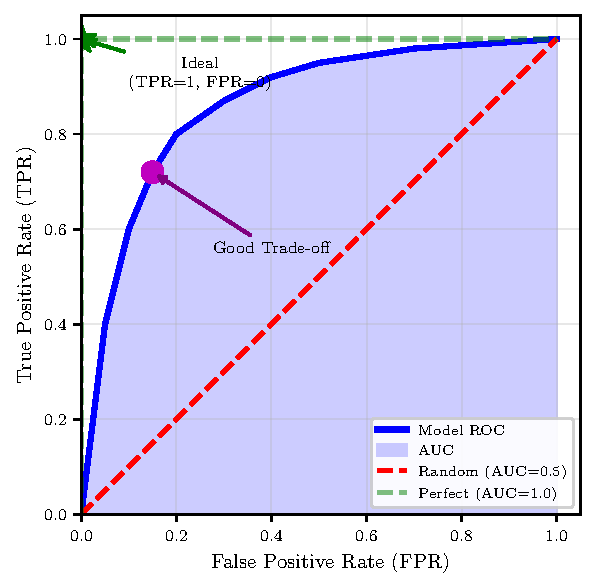
\includegraphics[width=\textwidth]{roc-curve-diagram.pdf}
\end{column}
\end{columns}
\end{frame}

\begin{frame}{Intuitive Understanding: TPR}
\begin{examplebox}{True Positive Rate (TPR)}
\small
$$\text{TPR} = \frac{\text{TP}}{\text{TP} + \text{FN}} = \frac{\text{TP}}{\text{All Actual Positives}}$$

\vspace{0.2cm}

\textbf{Question it answers:}
Of all actual brick kilns, what fraction did we detect?
\end{examplebox}

\vspace{0.15cm}

\begin{itemize}
    \item Same as Recall!
    \item Measures: Sensitivity of the detector
    \item High TPR = Catches most positives
    \item Low TPR = Misses many positives
\end{itemize}
\end{frame}

\begin{frame}{Intuitive Understanding: FPR}
\begin{examplebox}{False Positive Rate (FPR)}
\small
$$\text{FPR} = \frac{\text{FP}}{\text{FP} + \text{TN}} = \frac{\text{FP}}{\text{All Actual Negatives}}$$

\vspace{0.2cm}

\textbf{Question it answers:}
Of all non-kiln images, what fraction did we \\
incorrectly flag as having kilns?
\end{examplebox}

\vspace{0.15cm}

\begin{itemize}
    \item Measures: False alarm rate
    \item High FPR = Many false alarms
    \item Low FPR = Few false alarms
    \item FPR = $1 - $ Specificity
\end{itemize}
\end{frame}

\begin{frame}{The ROC Trade-off}
\begin{keypointsbox}{Fundamental Trade-off}
\small
As we vary the threshold:
\begin{itemize}
    \item Lower threshold $\rightarrow$ Higher TPR, Higher FPR
    \item Higher threshold $\rightarrow$ Lower TPR, Lower FPR
\end{itemize}
\end{keypointsbox}

\vspace{0.15cm}

\begin{columns}
\begin{column}{0.48\textwidth}
\begin{block}{Low Threshold}
\begin{itemize}
    \item Catch more positives
    \item But more false alarms
    \item Top-right of ROC
\end{itemize}
\end{block}
\end{column}

\begin{column}{0.48\textwidth}
\begin{block}{High Threshold}
\begin{itemize}
    \item Fewer false alarms
    \item But miss more positives
    \item Bottom-left of ROC
\end{itemize}
\end{block}
\end{column}
\end{columns}
\end{frame}

\begin{frame}{Building a ROC Curve: Steps}
\begin{enumerate}
    \item Train classifier, get predicted probabilities

    \vspace{0.15cm}

    \item For each threshold $\tau \in [0, 1]$:
    \begin{itemize}
        \item Apply threshold to get predictions
        \item Compute confusion matrix
        \item Calculate TPR and FPR
        \item Plot point (FPR, TPR)
    \end{itemize}

    \vspace{0.15cm}

    \item Connect points to form curve
\end{enumerate}
\end{frame}

\begin{frame}{Building a ROC Curve: Interpretation}
\begin{center}
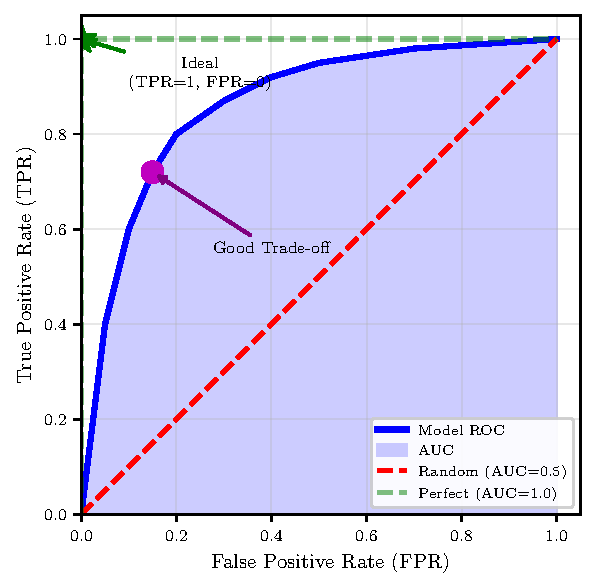
\includegraphics[width=0.6\textwidth]{roc-curve-diagram.pdf}
\end{center}

\begin{itemize}
    \item \textbf{Perfect classifier:} Curve hugs top-left corner
    \item \textbf{Random classifier:} Diagonal line
\end{itemize}
\end{frame}

\begin{frame}{Interpreting ROC Curves}
\begin{columns}
\begin{column}{0.48\textwidth}
\begin{keypointsbox}{Good ROC Curve}
\small
\begin{itemize}
    \item Closer to top-left
    \item Top-left = perfect!
    \item TPR=1, FPR=0
    \item High TPR, low FPR
\end{itemize}
\end{keypointsbox}

\begin{block}{Baselines}
\footnotesize
\begin{itemize}
    \item \textbf{Perfect:} Top-left
    \item \textbf{Random:} Diagonal
    \item \textbf{Bad:} Below diagonal
\end{itemize}
\end{block}
\end{column}
\begin{column}{0.48\textwidth}
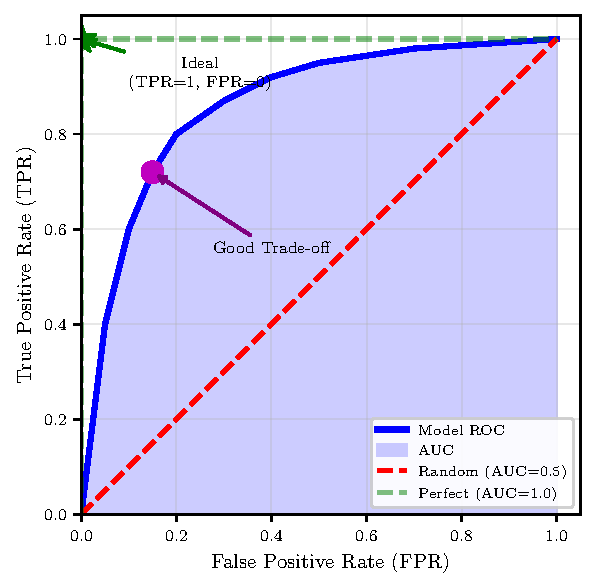
\includegraphics[width=\textwidth]{roc-curve-diagram.pdf}
\end{column}
\end{columns}
\end{frame}

\begin{frame}{Example: Same Dataset}
\begin{examplebox}{From Notebook}
\small
Using our Logistic Regression model
\end{examplebox}

\vspace{0.15cm}

\begin{center}
\small
\begin{tabular}{|c|c|c|}
\hline
\textbf{Threshold} & \textbf{TPR (Recall)} & \textbf{FPR} \\
\hline
0.00 & 1.00 & 1.00 \\
\hline
0.30 & 0.83 & 0.35 \\
\hline
0.50 & 0.69 & 0.23 \\
\hline
0.70 & 0.52 & 0.10 \\
\hline
0.90 & 0.24 & 0.00 \\
\hline
\end{tabular}
\end{center}

\vspace{0.15cm}

\begin{keypointsbox}{Observation}
\small
As threshold increases: TPR $\downarrow$, FPR $\downarrow$
\end{keypointsbox}
\end{frame}

\begin{frame}{AUC-ROC: Area Under ROC Curve}
\begin{columns}
\begin{column}{0.52\textwidth}
\begin{definitionbox}{AUC-ROC}
\small
Single number summarizing entire ROC curve

\vspace{0.2cm}
\footnotesize
$$\text{AUC-ROC} = \int_0^1 \text{TPR}(\text{FPR}) \, d(\text{FPR})$$

\vspace{0.2cm}

\textbf{Interpretation:}
\begin{itemize}
    \item Range: $[0, 1]$
    \item Perfect: AUC = 1.0
    \item Random: AUC = 0.5
    \item Higher is better
\end{itemize}
\end{definitionbox}
\end{column}
\begin{column}{0.48\textwidth}
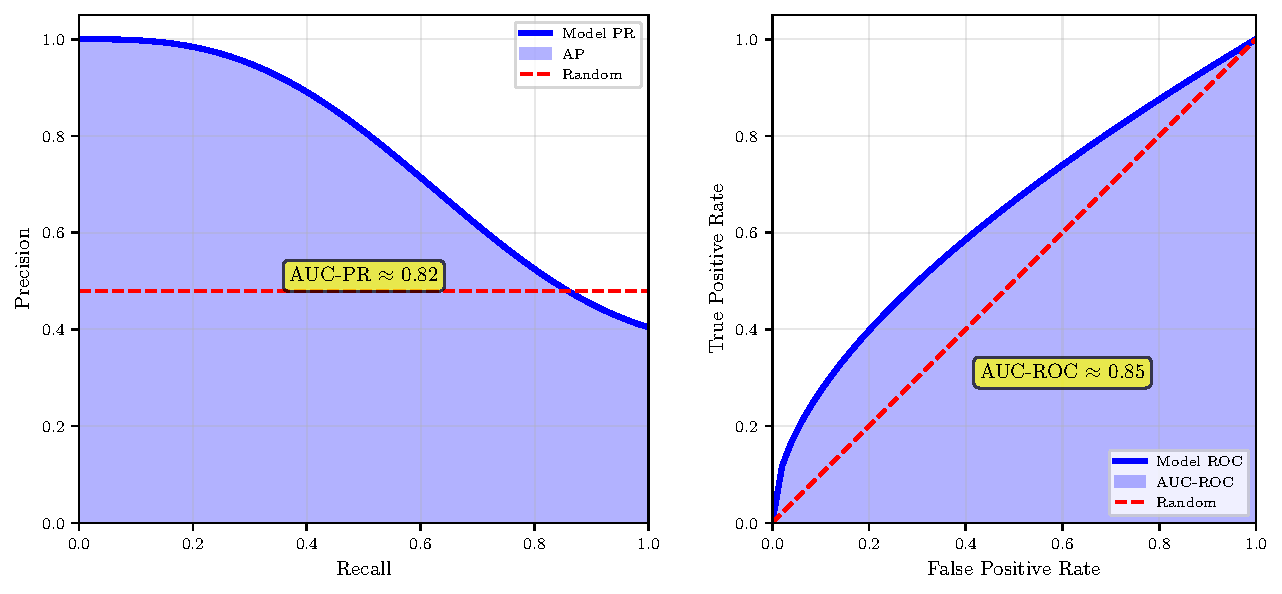
\includegraphics[width=\textwidth]{auc-diagram.pdf}
\end{column}
\end{columns}
\end{frame}

\begin{frame}{AUC-ROC Intuition}
\begin{keypointsbox}{Probabilistic Interpretation}
\small
AUC-ROC = Probability that the model ranks \\
a random positive example higher than \\
a random negative example
\end{keypointsbox}

\vspace{0.15cm}

\begin{examplebox}{Example}
\small
\begin{itemize}
    \item AUC = 0.95: 95\% chance model scores \\
          a true kiln higher than a non-kiln
    \item AUC = 0.50: Model is guessing randomly
    \item AUC = 0.85: Good discrimination ability
\end{itemize}
\end{examplebox}
\end{frame}

\begin{frame}[fragile]{ROC Implementation}
\begin{block}{Scikit-learn Implementation}
\small
\begin{verbatim}
from sklearn.metrics import (
    roc_curve, roc_auc_score,
    RocCurveDisplay
)

# Get predicted probabilities
y_scores = model.predict_proba(X_test)[:, 1]

# Compute ROC curve
fpr, tpr, thresholds = roc_curve(y_test, y_scores)
auc_roc = roc_auc_score(y_test, y_scores)

# Visualize
display = RocCurveDisplay(fpr=fpr, tpr=tpr,
                          roc_auc=auc_roc)
display.plot()
\end{verbatim}
\end{block}
\end{frame}

\begin{frame}{Comparing Multiple Models}
\begin{examplebox}{From Notebook: 3 Classifiers}
\small
\begin{itemize}
    \item Logistic Regression (linear boundary)
    \item Random Forest (non-linear, ensemble)
    \item SVM with RBF kernel (non-linear)
\end{itemize}
\end{examplebox}

\vspace{0.15cm}

\begin{center}
\begin{tabular}{|l|c|c|}
\hline
\textbf{Model} & \textbf{AUC-ROC} & \textbf{AUC-PR} \\
\hline
Random Forest & 0.92 & 0.90 \\
SVM (RBF) & 0.89 & 0.87 \\
Logistic Regression & 0.86 & 0.83 \\
\hline
\end{tabular}
\end{center}

\vspace{0.2cm}

\small
(Values approximate from notebook example)
\end{frame}

\section{PR vs ROC: When to Use Each}

\begin{frame}{Comparing PR and ROC Curves}
\begin{center}
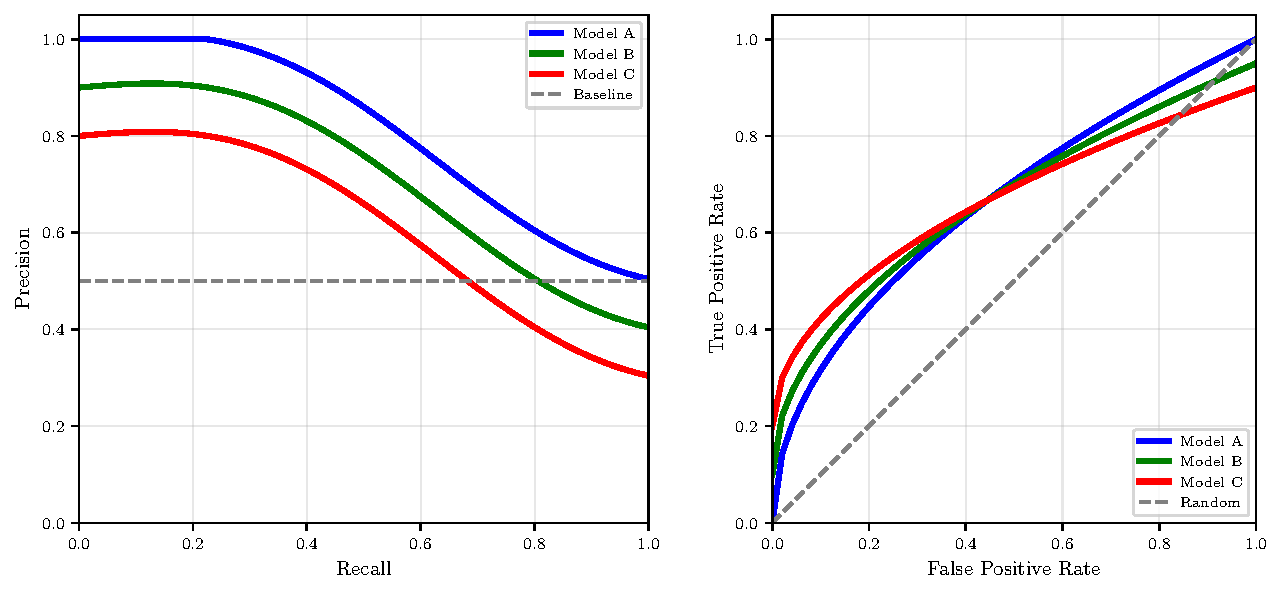
\includegraphics[width=0.95\textwidth]{model-comparison-diagram.pdf}
\end{center}

\vspace{0.2cm}

\begin{columns}
\begin{column}{0.48\textwidth}
\begin{block}{PR Curve}
\textbf{Plots:} Precision vs Recall \\
\textbf{Focus:} Positive class \\
\textbf{Sensitive to:} Imbalance
\end{block}
\end{column}

\begin{column}{0.48\textwidth}
\begin{block}{ROC Curve}
\textbf{Plots:} TPR vs FPR \\
\textbf{Focus:} Both classes \\
\textbf{Robust to:} Imbalance
\end{block}
\end{column}
\end{columns}
\end{frame}

\begin{frame}{Key Difference: Class Imbalance}
\begin{alertblock}{Critical Insight}
\small
ROC curves can be overly optimistic \\
on highly imbalanced datasets!
\end{alertblock}

\vspace{0.15cm}

\begin{examplebox}{Why?}
\small
FPR uses TN in denominator:
$$\text{FPR} = \frac{\text{FP}}{\text{FP} + \textcolor{red}{\text{TN}}}$$

With many negatives, even lots of FPs \\
can give a low FPR
\end{examplebox}
\end{frame}

\begin{frame}{Example: Imbalanced Data Setup}
\begin{examplebox}{Scenario: Highly Imbalanced Dataset}
\small
\begin{itemize}
    \item \textbf{Total images:} 1,000
    \item \textbf{Positive class} (has brick kilns): 50 (5\%)
    \item \textbf{Negative class} (no kilns): 950 (95\%)
\end{itemize}
\end{examplebox}

\vspace{0.2cm}

\begin{center}
\Large
This is a realistic scenario! \\
Many real-world problems have imbalanced classes
\end{center}
\end{frame}

\begin{frame}{Example: Imbalanced Data Analysis}
\begin{alertblock}{Model with 100 False Positives}
\footnotesize
Suppose our model produces 100 false alarms:

\vspace{0.15cm}

\textbf{Precision impact:}
\begin{itemize}
    \item Many false alarms per true positive
    \item Precision will be \textbf{low} (obvious problem!)
\end{itemize}

\vspace{0.15cm}

\textbf{FPR appears good:}
$$\text{FPR} = \frac{100}{100 + 850} = \frac{100}{950} = 0.105$$

Even with 100 false positives, FPR is only 10.5\%!
\end{alertblock}

\footnotesize
\begin{keypointsbox}{Conclusion}
\small
\textbf{PR curve:} Shows the problem clearly \\
\textbf{ROC curve:} Can hide issues in imbalanced data
\end{keypointsbox}
\end{frame}

\section{Practical Considerations}

\begin{frame}{PR Curves vs ROC Curves}
\begin{keypointsbox}{Use PR Curves When:}
\small
\begin{itemize}
    \item Classes are highly imbalanced
    \item You care primarily about positive class
    \item False positives and negatives differ in cost
\end{itemize}

\textbf{Examples:} Rare disease, fraud, information retrieval
\end{keypointsbox}

\vspace{0.15cm}

\begin{block}{Use ROC Curves When:}
\begin{itemize}
    \item Classes are relatively balanced
    \item Both classes equally important
\end{itemize}
\end{block}
\end{frame}

\begin{frame}{Why PR for Imbalanced Data?}
\begin{examplebox}{Brick Kiln Dataset}
\small
\begin{itemize}
    \item Total: 10,000 images
    \item Positive (has kiln): 150 (1.5\%)
    \item Negative (no kiln): 9,850 (98.5\%)
\end{itemize}
\end{examplebox}

\vspace{0.15cm}

\begin{alertblock}{Naive Classifier}
\small
Always predict ``no kiln'':
\begin{itemize}
    \item Accuracy: 98.5\% \textcolor{green}{(looks great!)}
    \item Precision: undefined
    \item Recall: 0\% \textcolor{red}{(useless!)}
\end{itemize}
\end{alertblock}
\end{frame}

\begin{frame}{The Problem with Accuracy}
\begin{keypointsbox}{Why Accuracy Fails}
\small
With extreme imbalance (1.5\% positive):
\begin{itemize}
    \item Accuracy dominated by majority class
    \item High accuracy doesn't mean good performance
    \item Need metrics focused on positive class
\end{itemize}
\end{keypointsbox}

\vspace{0.15cm}

\begin{center}
\Large
Use Precision, Recall, and PR curves!
\end{center}
\end{frame}

\begin{frame}[fragile]{Visualization with Scikit-learn}
\begin{block}{Complete Implementation}
\small
\begin{verbatim}
from sklearn.metrics import (
    precision_recall_curve,
    average_precision_score,
    PrecisionRecallDisplay
)

# Get scores
y_scores = model.predict_proba(X_test)[:, 1]

# Compute metrics
precision, recall, thresholds = \
    precision_recall_curve(y_test, y_scores)
ap = average_precision_score(y_test, y_scores)

# Visualize
display = PrecisionRecallDisplay(
    precision, recall, average_precision=ap)
display.plot()
\end{verbatim}
\end{block}
\end{frame}

\popquiz{
\textbf{
A model detects defective products (2\% of all products).
Your model achieves:
\begin{itemize}
    \item Precision: 0.60
    \item Recall: 0.90
\end{itemize}
Out of 10,000 products, how many will be flagged?}
\begin{enumerate}[A)]
    \item 150
    \item 300
    \item 600
    \item 900
\end{enumerate}
}{{\color{magenta}\textbf{B) 300}}}


\begin{frame}{Pop Quiz Answer}
\begin{examplebox}{Solution}
\small
\textbf{Answer: B) 300}
\end{examplebox}

\vspace{0.15cm}

\textbf{Step 1:} Actual defective products
$$10{,}000 \times 0.02 = 200$$

\textbf{Step 2:} True Positives (Recall = 0.90)
$$\text{TP} = 200 \times 0.90 = 180$$

\textbf{Step 3:} Use precision formula
$$0.60 = \frac{180}{\text{Total flagged}}$$
$$\text{Total flagged} = \frac{180}{0.60} = 300$$
\end{frame}

\popquiz{
\textbf{Which scenario needs model with Precision=0.70, Recall=0.85 over Precision=0.85, Recall=0.70?}

\begin{enumerate}[A)]
    \item Email spam detection \\
          (false positives lose legitimate mail)
    \item Airport security screening \\
          (missing threats is catastrophic)
    \item Credit card fraud \\
          (false positives block legitimate purchases)
    \item All equally
\end{enumerate}
}{{\color{magenta}\textbf{B) Airport security screening}}}

\begin{frame}{Pop Quiz Answer}
\begin{examplebox}{Solution}
\small
\textbf{Answer: B) Airport security screening}
\end{examplebox}

\vspace{0.15cm}

\textbf{Reasoning:}
\begin{itemize}
    \item First model has \textbf{higher recall (0.85)}
    \item Catches more true positives
    \item Missing a threat = catastrophic
    \item Better to have false alarms than miss threats
\end{itemize}

\vspace{0.15cm}

Options (a) and (c): False positives are costly \\
$\Rightarrow$ Need high precision
\end{frame}

\section{Summary}

\begin{frame}{Key Takeaways (1/2)}
\begin{keypointsbox}{Core Concepts}
\small
\begin{enumerate}
    \item \textbf{Precision:} Reliability of predictions
    \item \textbf{Recall:} Completeness of detection
    \item \textbf{Trade-off:} Can't maximize both
    \item \textbf{Thresholds:} Control the trade-off
\end{enumerate}
\end{keypointsbox}
\end{frame}

\begin{frame}{Key Takeaways (2/2)}
\begin{keypointsbox}{Practical Insights}
\small
\begin{enumerate}
    \setcounter{enumi}{4}
    \item \textbf{PR curves:} Show all trade-offs
    \item \textbf{Application:} Determines best point
    \item \textbf{Imbalanced data:} PR better than accuracy
    \item \textbf{Summary metrics:} F1, AP
\end{enumerate}
\end{keypointsbox}
\end{frame}

\begin{frame}{Workflow Summary}
\begin{enumerate}
    \item Train classifier
    \item Generate PR curve on validation set
    \item Analyze precision-recall trade-offs
    \item Choose threshold based on:
    \begin{itemize}
        \item Application requirements
        \item Cost of errors
        \item Available resources
    \end{itemize}
    \item Validate on test set
    \item Monitor in production
    \item Adjust if requirements change
\end{enumerate}
\end{frame}

\begin{frame}{The Right Model for YOUR Application}
\begin{center}
\Large
The best model makes the right trade-offs \\
for \textbf{your specific application}

\vspace{0.2cm}

Not the highest accuracy, \\
not the highest F1, \\
but the one that aligns with your goals!
\end{center}
\end{frame}

\begin{frame}{Further Resources}
\begin{itemize}
    \item \textbf{Notebook:} \href{https://nipunbatra.github.io/ml-teaching/notebooks/pr-curve.html}{\texttt{pr-curve.html}} \\
          Running example with visualization code

    \item \textbf{Documentation:} \\
          Scikit-learn Precision-Recall guide

    \item \textbf{Related topics:}
    \begin{itemize}
        \item ROC curves and AUC
        \item Cost-sensitive learning
        \item Threshold optimization
        \item Multi-class metrics
    \end{itemize}
\end{itemize}
\end{frame}

\begin{frame}
\begin{center}
\Huge
Thank you!

\vspace{1cm}

\Large
Questions?
\end{center}
\end{frame}

\end{document}
